\documentclass[11pt,a4paper]{article}
\usepackage[T1]{fontenc}
\usepackage[utf8]{inputenc}
\usepackage{lmodern}
\usepackage{amsmath,amssymb,amsthm}
\usepackage{booktabs}
\usepackage{array}
\usepackage{graphicx}
\usepackage[margin=2.5cm]{geometry}
\usepackage{hyperref}
\hypersetup{colorlinks=true,linkcolor=blue,citecolor=blue,urlcolor=blue}
\graphicspath{{../figures/}}

\newtheorem{proposition}{Proposition}
\newtheorem{lemma}{Lemma}
\newtheorem{assumption}{Assumption}
\theoremstyle{remark}
\newtheorem{remark}{Remark}

% ---- operators
\newcommand{\wrap}{\operatorname{wrap}}
\newcommand{\med}{\operatorname{med}}
\newcommand{\cmed}{\operatorname{med}^{\circ}}
\newcommand{\E}{\mathbb{E}}
\newcommand{\Var}{\operatorname{Var}}
\newcommand{\Cov}{\operatorname{Cov}}
\newcommand{\sgn}{\operatorname{sgn}}
\newcommand{\dg}{^{\circ}}
\newcommand{\code}[1]{\texttt{#1}}
% ---- directions
\newcommand{\Wt}{W_{\mathrm{t}}}
\newcommand{\Nt}{N_{\mathrm{t}}}
\newcommand{\Wr}{W_{\mathrm{r}}}
\newcommand{\Nr}{N_{\mathrm{r}}}


\title{Static yaw misalignment from high-resolution SCADA:\\
       the label-free (T0) method, step by step}
\author{Nadara / WeDoWind challenge, participant 33}
\date{October 2026}

\begin{document}
\maketitle

\begin{abstract}
\sloppy
This note derives the label-free (tier T0) method behind
\code{Results\_33\_T0\_0.csv} (\code{PPP\_WTG17}) and
\code{Results\_33\_T0\_final.csv} (\code{SSS\_WTG06}). It is the T0 part of the
complete derivation note of the project: every operation performed on the data
is described in the order in which it is performed, with the exact thresholds
that the code uses. Section~\ref{sec:notation} fixes the notation,
\S\ref{sec:step1} covers reconstruction and cleaning, \S\ref{sec:sensor} the
sensor model, \S\ref{sec:step2} the neighbour residual and the states,
\S\ref{sec:step4} the submission model, \S\ref{sec:scoring} the scoring rule and
\S\ref{sec:summary} the assumptions. The method fits no parameter to labels;
\S\ref{sec:labeluse} states exactly where labels were looked at. The code
that implements the method is in \code{src/yaw/} and \code{scripts/} of this
repository.
\end{abstract}

\tableofcontents

%======================================================================
\section{Notation}\label{sec:notation}

\subsection{Conventions}
All directions are compass bearings in degrees, clockwise from north. A difference
of two bearings is always wrapped to $[-180\dg,180\dg)$,
\begin{equation}
  \wrap(x) = \big((x+180) \bmod 360\big) - 180 .
  \label{eq:wrap}
\end{equation}

Time has three resolutions. The raw stream is sampled at roughly $12$\,s; a raw
sample is indexed by $t$. Minute aggregates are indexed by $m$ (1-minute bins) or
$m_{10}$ (10-minute bins). Calendar days are indexed by $d$. Turbines are indexed
by $i$ (the target) and $j$ (a neighbour). A contiguous run of days with constant
behaviour is a \emph{state}, indexed by $\ell$.

For a set of bearings $x_1,\dots,x_n$ the \emph{circular mean} and the
\emph{mean resultant length} are
\begin{equation}
  \bar x = \operatorname{atan2}\Big(\tfrac1n\sum_i \sin x_i,\ \tfrac1n\sum_i \cos x_i\Big),
  \qquad
  \bar R = \Big|\tfrac1n\sum_i e^{\mathrm{i}x_i}\Big| \in [0,1],
  \label{eq:circmean}
\end{equation}
where $\bar R = 1$ means all bearings are equal and $\bar R\to0$ means they are
spread around the circle. The \emph{circular median} is the ordinary median of the
wrapped deviations from the circular mean,
\begin{equation}
  \cmed(x) = \bar x + \med_i \wrap(x_i - \bar x) .
  \label{eq:circmed}
\end{equation}
It inherits the robustness of the median and does not depend on where the
$\pm180\dg$ cut sits. $\med$ without subscript is the ordinary median.

\subsection{Symbols}
Table~\ref{tab:symbols} lists every symbol used in the note. Physical quantities
that carry the undisclosed scale factor of the data set (power, wind speed,
rotor and generator speed, pitch) are only ever used in ratios, differences or
threshold comparisons, never as absolute physical values.

\begin{table}[h]\centering\small
\begin{tabular}{@{}>{$}l<{$}p{11.5cm}@{}}
\toprule
\multicolumn{2}{@{}l}{\emph{Reported SCADA channels (per raw sample $t$)}}\\
P & active power (scaled units; rated $P_{\mathrm{rated}}\approx4800$)\\
U & nacelle-anemometer wind speed (scaled)\\
\Omega,\ \Omega_g & rotor and generator speed (scaled)\\
\varphi & blade pitch angle (degrees)\\
\Nr & reported nacelle heading, field \code{NacDir}\\
\Wr & reported wind direction, field \code{WindDir}\\
v & reported vane angle, derived: $v=\wrap(\Wr-\Nr)$\\
\midrule
\multicolumn{2}{@{}l}{\emph{Physical (unobserved) quantities}}\\
\Wt & true free-stream wind direction at the rotor\\
\Nt & true nacelle heading (rotor axis)\\
\gamma & instantaneous yaw error $\gamma=\wrap(\Wt-\Nt)$, positive when the wind comes from clockwise of the rotor axis\\
\theta & static yaw misalignment $\theta=\E[\gamma]$ over a day or a state; the label\\
\delta_n,\ \delta_v & mounting offsets of the nacelle encoder and of the wind vane\\
g & gain of the vane ($g\le1$); the implementation uses $g=1$\\
s & vane set-point of the yaw controller\\
\midrule
\multicolumn{2}{@{}l}{\emph{Consensus and states}}\\
D_{ij} & heading difference of a pair, $D_{ij}=\wrap(\Nr^i-\Nr^j)$\\
J & size of a level shift in a pair series\\
m_{ij}(\cdot) & sector median of $D_{ij}$ in the neighbour's wind-direction sector\\
\kappa & unknown constant of the consensus (\S\ref{sec:algebra})\\
r_i(d) & daily consensus heading residual of turbine $i$\\
\tilde r_i(d) & its 7-day rolling median\\
\bar r_\ell & level of state $\ell$ (median of $\tilde r$ over the state)\\
\lambda,\ n_{\min} & change-point penalty and minimum state length of PELT\\
\midrule
\multicolumn{2}{@{}l}{\emph{Submission}}\\
L & level prior of a turbine (vane set-point)\\
\alpha & anchor of an encoder-free segment\\
x & centred state level $x=\bar r_\ell-\alpha$\\
\bottomrule
\end{tabular}
\caption{Symbols. Hats denote estimates, bars denote means or levels.}
\label{tab:symbols}
\end{table}

%======================================================================
\section{Reconstruction, cleaning and aggregation}\label{sec:step1}
\subsection{The change-based stream}
The parquet files hold one row per turbine and timestamp with seven channels
($P$, $U$, $\Omega$, $\Omega_g$, $\varphi$, $\Nr$, $\Wr$). The stream is
\emph{change-based}: a channel is written only when its value changed, and a
null means ``unchanged since the previous row'', not ``missing''. Per channel
the fraction of written rows is $0.5$--$0.8$, except $\Nr$, which is written on
only $\approx6\,\%$ of rows because the nacelle moves only during yaw
manoeuvres.

\paragraph{Reconstruction rule.} Rows are sorted by (turbine, $t$). Before
filling, the indicator
\begin{equation}
  u_t = \mathbf 1[\Nr \text{ written at } t]
  \label{eq:nac_update}
\end{equation}
is kept: it marks a \emph{yaw controller action} and is lost after filling.
Then every channel is forward-filled per turbine (\code{ffill}), so that each
row carries the last known value of every channel. Nothing is interpolated;
a value holds until the next write.

\paragraph{The vane.} The vane angle is not shipped. In this SCADA the wind
direction field is computed by the controller as heading plus vane, so
\begin{equation}
  v_t = \wrap(\Wr - \Nr)_t
  \label{eq:vane}
\end{equation}
returns the vane reading exactly (checked on the raw pairs).
Consequently $\Wr$ carries whatever offset the nacelle encoder carries, and only
$v$ is encoder-free. This single fact shapes the whole pipeline
(\S\ref{sec:sensor}).

\paragraph{Asynchronous writes (a trap).} Because $\Nr$ and $\Wr$ are written
independently, at a row where $\Nr$ was just updated the filled $\Wr$ still holds
the value computed at the \emph{previous} $\Wr$ write. Equation~\eqref{eq:vane}
then reads $v^{\mathrm{old}} - \Delta$ (with $\Delta$ the heading change) until
$\Wr$ refreshes, whatever the physical vane does. Nothing at the 12-second
scale may therefore use $v$ across a heading update; see \S\ref{sec:gain}.

\subsection{Aggregation with circular statistics}\label{sec:agg}
The filled stream is binned to 1-minute and 10-minute bins. For a bin containing
raw samples $t\in m$:
\begin{itemize}
\item linear channels ($P,U,\Omega,\Omega_g,\varphi,v$): the mean $\bar P_m$, etc.;
      in addition the within-bin standard deviation of $P$, $U$ and $v$, and the
      median $v^{\med}_m$ of the vane;
\item directions ($\Nr,\Wr$): the circular mean \eqref{eq:circmean} and the
      resultant length $\bar R_m$; a naive mean of $350\dg$ and $10\dg$ would be
      $180\dg$, and several turbines spend much time near north;
\item counts: number of raw rows $n_m$, number of controller actions
      $\sum_{t\in m} u_t$, and the operating fraction
      $\omega_m = \frac1{n_m}\sum_{t\in m}\mathbf 1[P_t > P_{\min}]$.
\end{itemize}
Per turbine this gives $\approx1.0\times10^6$ minutes from $4.7$--$5.9\times10^6$
raw rows over the $727$--$731$ days of record.

\subsection{Operating regime}\label{sec:regimes}
The undisclosed scale factor forbids physical thresholds; the thresholds are
therefore set from the data. The $99.9$th percentile of $P$ defines
$P_{\mathrm{rated}} = 4800$. A minute is
\begin{equation}
  \text{operating} \iff \bar P_m > P_{\min} = 100 \quad(\approx2\,\% \text{ of rated}).
  \label{eq:regime}
\end{equation}
This is the only use of power in the T0 method.

\subsection{Daily table and sensor-health flags}\label{sec:health}
Per turbine and day the minutes are summarised: number of minutes, rows and
controller actions, operating minutes, and, over the
\emph{operating} minutes only, the daily median vane
\begin{equation}
  v^{\med}_d = \med_{m\in d,\ \text{operating}} v^{\med}_m ,
  \label{eq:vane_daily}
\end{equation}
its inter-quartile range, the mean within-minute vane standard deviation, the
median pitch and rotor speed, and the circular mean heading. Three flags mark
days that no estimator may use:
\begin{align*}
  \text{frozen vane} &: \text{mean within-minute vane std} < 0.05\dg \ \wedge\ \text{operating minutes} > 60,\\
  \text{no yaw}      &: \textstyle\sum_d u_t = 0 \ \wedge\ \text{operating minutes} > 60,\\
  \text{sparse}      &: \text{raw rows} < 1000 .
\end{align*}
A day is \emph{healthy} when none of the three is set. The flags catch two real
faults: \code{PPP\_WTG13} reports $v=-34.0\dg$ with zero variance and no
controller action on 8--16 Feb 2024 and $v=+39.1\dg$ on 9--12 Oct 2024 (11 and 7
days); no other turbine has a frozen vane. Sparse days are $1$--$8$ per turbine.

\subsection{Labels and label-derived states}\label{sec:labels}
The label $\theta^\star_d$ is given per row of the training turbines and is
constant within a day; the daily series is its first value per day
($195$, $312$ and $195$ labelled days on \code{PPP\_WTG12/13/14}, January to
November 2023). The organisers score only days outside a transition window
around each label step, but do not publish the window rule; it is reconstructed
as follows. The daily label series of each turbine is segmented into
piecewise-constant states with the PELT algorithm (\S\ref{sec:pelt}) under an
$L_2$ cost with penalty $\lambda=20$ and minimum length $n_{\min}=7$ days. The
state level is the median label within the state. A day is a \emph{transition}
when it lies within $7$ calendar days of a state boundary (gaps count as days)
or when its label deviates by more than $0.75\dg$ from its state level; a day is
\emph{scored} when it is labelled and not a transition. This gives $2$, $6$ and
$2$ states and $180$, $217$ and $180$ scored days. All local scoring
(\S\ref{sec:scoring}) uses this table.

\subsection{Layout and neighbours}\label{sec:layout}
The layout files give coordinates with an unknown common scale, so distances are
only used as ratios and bearings are exact. The neighbours of turbine $i$ are
the same-site turbines sorted by distance.

\subsection{Pair offsets}
For every same-site pair $(i,j)$ and every 10-minute bin in which both turbines
operate more than $90\,\%$ of the bin ($\omega_{m_{10}}>0.9$ for both), the
heading difference $D_{ij}=\wrap(\Nr^i-\Nr^j)$ and the wind-direction
difference $\wrap(\Wr^i-\Wr^j)$ are formed, and their daily medians and
inter-quartile ranges are stored ($65$ pairs). This table is diagnostic
(Figure~\ref{fig:vane}); the consensus of \S\ref{sec:step2}
recomputes the pair series with a circular median.

\begin{figure}[p]\centering
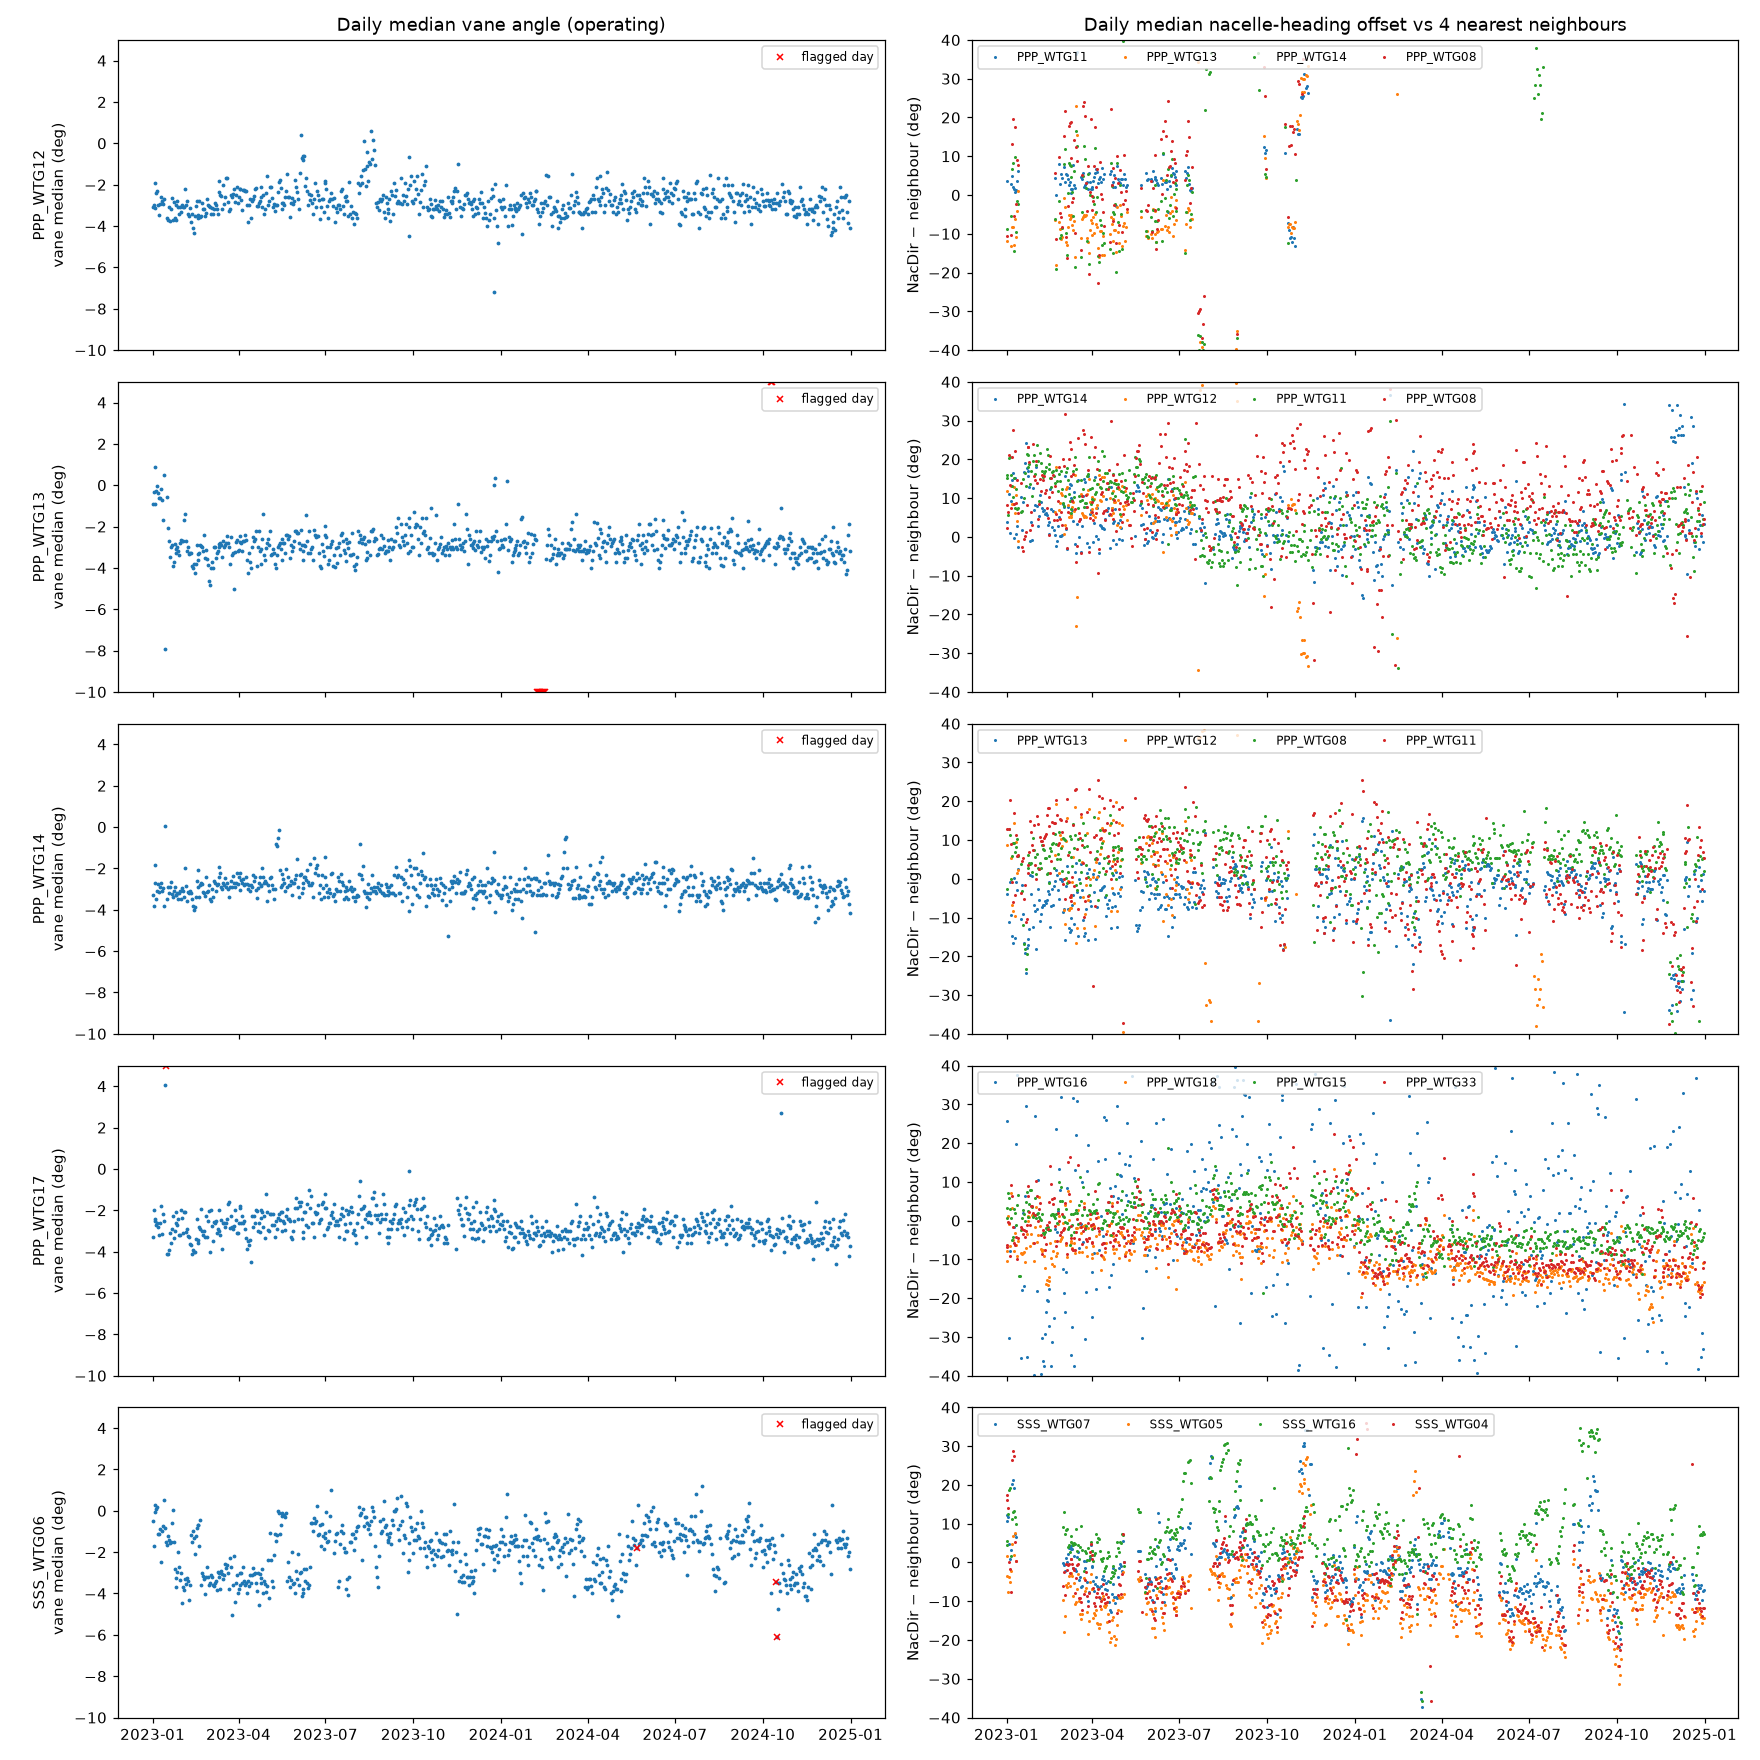
\includegraphics[width=\textwidth]{01_vane_and_offsets.png}
\caption{Left: daily median vane angle in operation, $v^{\med}_d$. Right: daily
median heading offset $D_{ij}$ to the four nearest neighbours, before
de-stepping and cleaning.}
\label{fig:vane}
\end{figure}

\subsection{What the cleaning revealed}
Three facts from this step drive the design:
\begin{enumerate}
\item \textbf{The vane set-point is not zero.} On every PPP turbine the daily
      median vane in operation is $-2.7\ldots-3.7\dg$; on SSS it is $-0.8$ or
      $-3.1\dg$, and \code{SSS\_WTG06} wanders between $0$ and $-4\dg$ over
      weeks. The controller nulls the vane at $\approx-3\dg$, not at $0$.
\item \textbf{Encoders lose north.} \code{PPP\_WTG12}'s heading jumps by
      $\approx138\dg$ against every neighbour from August 2023 while its label does
      not move; on $10$--$17\,\%$ of days a turbine of the WTG12/13/14 cluster sits
      $100$--$180\dg$ away from all neighbours for several days while producing
      normally. These are encoder-frame events, not flow.
\item \textbf{Labels and vane can move in opposite directions.} On
      \code{PPP\_WTG13} the vane median moved from $\approx-0.5$ to $\approx-3\dg$
      on 14--18 January 2023 while the label went from $-11.5$ to $-8.1\dg$. This
      becomes the sign check of \S\ref{sec:signcheck}.
\end{enumerate}

%======================================================================
\section{The sensor model}\label{sec:sensor}

\subsection{True and reported quantities}
At any instant the unobserved quantities are the true wind direction $\Wt$, the
true nacelle heading $\Nt$ and the yaw error $\gamma=\wrap(\Wt-\Nt)$. The stream
reports
\begin{align}
  \Nr &= \Nt + \delta_n, \label{eq:Nr}\\
  v   &= g\,\gamma + \delta_v, \label{eq:v}\\
  \Wr &= \Nr + v . \label{eq:Wr}
\end{align}
Equation~\eqref{eq:Nr} says the encoder has no north reference: $\delta_n$ is an
arbitrary constant that changes at every re-reference. Equation~\eqref{eq:v}
says the vane measures the yaw error with a mounting offset $\delta_v$ and a gain
$g\le1$; the gain models the well-documented damping of the inflow angle behind a
rotating rotor (wake swirl, nacelle body).\footnote{Everything below is written
for general $g$; the implementation uses $g=1$ because \S\ref{sec:gain} shows $g$
cannot be measured from this data.} Equation~\eqref{eq:Wr} is not an
assumption but the encoding of the data set, \S\ref{sec:step1}.

\subsection{The controller and the definition of the label}
The yaw controller filters $v$ over minutes and rotates the nacelle whenever the
filtered reading leaves a deadband (measured occupancy $\approx\pm8\dg$) around
its set-point $s$. In steady state the controller therefore enforces
$\E[v]=s$, and from \eqref{eq:v}
\begin{equation}
  \theta \;\equiv\; \E[\gamma] \;=\; \frac{s-\delta_v}{g}.
  \label{eq:theta_def}
\end{equation}
$\theta$ is the \emph{static yaw misalignment}: the persistent yaw error the
controller cannot see because it sits inside its own measurement. The WindFit
reference system measures it with an independent sensor and fits the
power-optimal heading over several days, which is why its daily series is
smoothed and drifts for about a week before each step, and why days near a step
are not scored. The label is negative on all three training turbines; the
sign check of \S\ref{sec:signcheck} establishes that the label sign coincides
with $\gamma$ as defined here.

Two consequences shape everything that follows.
\begin{enumerate}
\item \textbf{The vane cannot see $\theta$.} Averaged over any window the vane
      reads $s$ whatever $\theta$ is. Measured: $v^{\med}_d\approx-3\dg$ on
      every PPP turbine irrespective of the label (correlation with the label
      $-0.33$). Information about $\theta$ must come from the \emph{response} of
      the turbine to $\gamma$ (power) or from an external direction reference
      (neighbours). The T0 method uses the neighbours.
\item \textbf{$\theta$ changes in three ways} that the sensors do not treat
      alike: a change of the set-point $s$, of the vane offset $\delta_v$, or of
      the gain $g$. All three move $\theta$ by \eqref{eq:theta_def}; only the
      first two move the neighbour residual of \S\ref{sec:step2}; and an encoder
      re-reference ($\delta_n$) moves the residual without moving $\theta$ at
      all.
\end{enumerate}

\subsection{Why the vane gain cannot be measured here}\label{sec:gain}
If the vane responded instantaneously with gain $g$, a nacelle rotation $\Delta$
during steady wind would produce a vane jump of $-g\Delta$ (\eqref{eq:v} with
$\gamma\to\gamma-\Delta$), and the thousands of manoeuvres would give $g$
directly. On this data
the derived vane jumps by \emph{exactly} $-\Delta$ at every heading update. The
reason is the asynchronous encoding described in \S\ref{sec:step1}: at a
heading update $\Wr$ still holds $\Nr^{\mathrm{old}}+v^{\mathrm{old}}$, so
\eqref{eq:vane} reads $v^{\mathrm{old}}-\Delta$ until $\Wr$ refreshes, whatever
the vane does. The apparent gain is one by construction, and no quantity derived
from the two direction channels at the 12-second scale can recover $g$. Therefore
$g=1$ is used throughout.

%======================================================================
\section{Encoder frames, consensus residual and states}\label{sec:step2}
\subsection{Sensor algebra of the residual}\label{sec:algebra}
Suppose a consensus estimate $c(t)$ of the true wind direction is available from
the neighbours, of the form $c = \Wt + \kappa$ with $\kappa$ a constant that
depends on the neighbours' own offsets. From \eqref{eq:Nr} and
$\gamma=\Wt-\Nt$,
\begin{equation}
  \wrap(\Nr - c) = \Nt + \delta_n - \Wt - \kappa = -\gamma + \delta_n - \kappa .
  \label{eq:residual}
\end{equation}
Averaged over a day, $\E[\gamma]=\theta$, so the daily residual obeys
\begin{equation}
  \boxed{\ r(d) = -\theta(d) + \delta_n(d) - \kappa\ }
  \qquad\Longrightarrow\qquad
  \Delta r = -\Delta\theta \quad\text{whenever } \Delta\delta_n = 0 .
  \label{eq:dr}
\end{equation}
\begin{proposition}\label{prop:residual}
The residual identifies \emph{changes} of the static misalignment in physical
degrees with slope exactly $-1$, independent of the vane ($g$, $\delta_v$) and
of the aerodynamics; its \emph{level} is not identifiable, because $\delta_n$
and $\kappa$ are unknown constants.
\end{proposition}
\noindent This is the ``consensus anchor'' of the leading team. Using $\Wr$
instead of $\Nr$ gives $\Wr - c = \delta_n + \delta_v + (g-1)\gamma - \kappa$,
a constant for $g=1$ and a damped version of \eqref{eq:dr} for $g<1$; the
implementation uses $\Nr$. The residual is blind to changes of $\theta$ that
occur through $g$ (the wind side of $\gamma$ does not move), but such changes
are also invisible to the label mechanism to first order.

The consensus $c$ is never formed explicitly. Instead the residual is built pair
by pair, \S\ref{sec:cons_build}, which is equivalent because every pair
difference $D_{ij} = \wrap(\Nr^i-\Nr^j)$ contains $-\gamma^i+\gamma^j+\delta_n^i-\delta_n^j$
and the neighbour's terms are constant over a day up to noise.

\subsection{Pair series, excursions and re-references}\label{sec:destep}
$\delta_n$ is piecewise constant with jumps. A jump of $\delta_n^i$ moves
$D_{ij}$ against \emph{all} neighbours $j$ by the same amount on the same day;
the detection rule uses exactly this signature. Two kinds of jump occur and
must be treated differently: a \emph{re-reference}, after which $\delta_n$
stays at its new value, and an \emph{excursion}, in which the heading reads of
the order of $100\dg$ off for one to six weeks and then returns to the old
frame. Excursions are by far the more frequent.

\paragraph{Reference set.} For each turbine $i$ the $n_{\mathrm{nb}}=4$ nearest
same-site turbines are its references, excluding \code{PPP\_WTG12} and
\code{PPP\_WTG16}, whose headings are too unstable to serve as references (they
still receive their own residual from the remaining neighbours).

\paragraph{Daily pair series.} From the 10-minute aggregates, for bins where both
turbines operate more than $90\,\%$ of the time,
\begin{equation}
  D_{ij}(d) = \cmed_{m_{10}\in d}\ \wrap\big(\Nr^i - \Nr^j\big)_{m_{10}} .
  \label{eq:pair_daily}
\end{equation}

\paragraph{Level shifts.} Each daily pair series is unwrapped (so that a
crossing of $\pm180\dg$ is not read as a jump) and segmented with PELT under an
$L_1$ cost, penalty $\lambda=150$, minimum length $n_{\min}=10$ days
(\S\ref{sec:pelt}). The $L_1$ cost (median per segment) is chosen so that single
outlying days do not create segments. Each boundary yields a candidate jump
$J$, the wrapped difference of the medians of the adjacent segments.

\paragraph{Attribution rule.} A candidate jump on date $d$ in the series
$(i,j)$ is credited to the encoder of $i$ when candidates with $|J|\ge25\dg$ of
the same sign appear within $\pm3$ days in at least $60\,\%$ of $i$'s pairs and
in at least two of them. The credited jump is the median of the matching
candidates and its date the earliest of them. Shifts below $25\dg$ cannot be
attributed by majority: a $5\dg$ misalignment change and a $5\dg$
re-reference look identical in every pair. Fifty-nine steps on nine turbines
were credited, none on \code{PPP\_WTG17} or its three nearest neighbours.

\paragraph{Why the credited jumps are not subtracted.} The first version of
the method subtracted every credited jump $J_n$ from the heading from its date
on. For an excursion this subtracts two independent estimates, one out and one
back, each a difference of medians of whole PELT segments of which the
excursion segment holds only $10$--$20$ noisy days. They do not cancel: on
\code{SSS\_WTG06} the pairs $(-92.2,+101.9)$, $(-119.2,+125.7)$,
$(-111.0,+112.4)$ and $(-108.9,+117.3)$ leave $+9.6$, $+6.5$, $+1.5$ and
$+8.4\dg$ in $r$, and a one-week deviation in November 2023 was credited as a
single $-30.3\dg$ step with no return. These remainders are as large as the
misalignment signal of \eqref{eq:dr} and produced $13$ states on
\code{SSS\_WTG06} where the raw pair offsets show three. The validate turbine
has no credited step and was unaffected, so the defect was invisible in the
validate round.

\paragraph{Frame plan.} The credited step dates $d_1<d_2<\dots$ of turbine $i$
cut its record into intervals; the jump sizes $J_n$ are not used further.
\begin{enumerate}
\item An interval shorter than $45$ days is an \emph{excursion}. Its days are
      dropped, together with $\pm3$ days around every step date. Nothing is
      subtracted.
\item For two consecutive long intervals $A$ (before) and $B$ (after) the
      shift is measured \emph{locally},
      \begin{equation}
        J_{AB} = \med_j\ \wrap\big(\bar D_{ij}^{B} - \bar D_{ij}^{A}\big),
        \qquad
        \bar D_{ij}^{B} = \cmed_{d\in B_{40}} D_{ij}(d),\quad
        \bar D_{ij}^{A} = \cmed_{d\in A_{40}} D_{ij}(d),
        \label{eq:localjump}
      \end{equation}
      with $B_{40}$ the first $40$ days of $B$ and $A_{40}$ the last $40$ days
      of $A$,
      on the raw daily pair series \eqref{eq:pair_daily}, with a margin of $3$
      days at the interval edges, at least $7$ days on each side, and without
      the days within $25$ days of a credited step of the neighbour $j$.
\item If $|J_{AB}|<15\dg$ the frame \emph{came back}: no correction is applied,
      and whatever small difference remains between $A$ and $B$ is left in the
      data as signal.
\item If $|J_{AB}|\ge15\dg$ the shift is a \emph{re-reference}: from the start
      of $B$ on, both direction channels are corrected,
      \begin{equation}
        \Nr^{i}(t) \leftarrow \big(\Nr^{i}(t) - J_{AB}\big) \bmod 360,
        \qquad \text{and likewise } \Wr^{i},
        \label{eq:destep}
      \end{equation}
      cumulatively over successive re-references, and the date is recorded.
\end{enumerate}
$\Wr$ must be corrected too because it carries $\delta_n$ by \eqref{eq:Wr}; $v$
is unaffected. The plan finds $37$ excursions on eight turbines, $10$ to $43$
days long ($117$ days in seven excursions on \code{SSS\_WTG06}, $123$ on
\code{SSS\_WTG04}, $148$ on \code{PPP\_WTG14}), and a single re-reference:
\code{PPP\_WTG12} on 2023-07-28, $J_{AB}=147\dg$. The rule assumes that the
misalignment does not change by $15\dg$ or more across an excursion; a change
below that survives, a change above it would be removed as a re-reference.

\subsection{Building the residual}\label{sec:cons_build}
After the frame plan has been applied, three cleaning operations and one
correction are applied to each pair before the residual is formed.
\begin{enumerate}
\item \textbf{Transient removal.} The daily pair series \eqref{eq:pair_daily}
      is recomputed on the corrected headings and compared with its centred
      rolling median over 91 days with data (at least 7 present; gaps are skipped, so the window can span more calendar days). Days with
      $|\wrap(D_{ij}(d) - \text{rolling median})| > 10\dg$ are dropped from the
      pair. A rolling median reproduces a level shift of any size exactly but
      suppresses a pulse shorter than half its window, so this removes the
      excursions, of the target \emph{or} of the neighbour, that are too small
      or too short to be credited in \S\ref{sec:destep} (two of about $18\dg$
      on \code{SSS\_WTG06}), while a persistent step passes unchanged. The
      price is that a real state shorter than about $45$ days which departs by
      more than $10\dg$ and returns is removed as well. Lowering the
      $25\dg$ attribution threshold to $12\dg$ instead was tried and did not
      catch these excursions.
\item \textbf{Sector correction.} Terrain steering and partial wakes make the
      direction difference between two sites a function of the wind direction.
      With $\sigma_j$ the $30\dg$ sector of the neighbour's (de-stepped) wind
      direction, $\sigma_j = \lfloor \Wr^j / 30\dg\rfloor$, the sector median
      $m_{ij}(\sigma_j) = \cmed\{D_{ij}(m_{10}) : \text{bins in sector } \sigma_j\}$
      is subtracted bin by bin,
      \begin{equation}
        e_{ij}(m_{10}) = \wrap\big(D_{ij}(m_{10}) - m_{ij}(\sigma_j(m_{10}))\big) .
        \label{eq:sector}
      \end{equation}
      The neighbour's wind direction is used as the sector variable because it
      is not affected by the target's own yaw error.
\item \textbf{Daily pair residual.} $e_{ij}(d) = \med_{m_{10}\in d} e_{ij}(m_{10})$
      over days with at least $12$ valid bins; its daily inter-quartile range is
      kept as a noise measure.
\item \textbf{Noisy references.} A pair whose median daily inter-quartile range
      exceeds twice the median of the turbine's pairs is dropped.
\end{enumerate}
The daily residual of turbine $i$ is the median over the surviving pairs,
\begin{equation}
  r_i(d) = \med_{j}\ e_{ij}(d) .
  \label{eq:r_def}
\end{equation}
The double median (over bins, then over neighbours) makes \eqref{eq:r_def}
robust to one bad neighbour and to a few bad bins; the measured day-to-day
noise is $\approx2\dg$ (median absolute deviation). The price is that changes
below $\approx1\dg$, the two small label steps on WTG12 and WTG14, are under the
noise floor. In terms of \S\ref{sec:algebra}, the sector medians $m_{ij}$
absorb $\delta_n^j$, $\theta^j$ and the terrain term into the constant $\kappa$,
and $r_i$ is \eqref{eq:dr} up to that constant.

\subsection{Change-point detection: PELT}\label{sec:pelt}
Both the label states (\S\ref{sec:labels}), the encoder steps
(\S\ref{sec:destep}) and the SCADA states (\S\ref{sec:states}) use the same
algorithm. Given a series $y_1,\dots,y_T$, a partition into contiguous segments
$\mathcal S_1,\dots,\mathcal S_M$ is chosen to minimise
\begin{equation}
  \sum_{\ell=1}^{M}\ C(\mathcal S_\ell) \;+\; \lambda\,(M-1),
  \qquad |\mathcal S_\ell| \ge n_{\min},
  \label{eq:pelt}
\end{equation}
with the segment cost either
\begin{equation}
  C_{L_2}(\mathcal S) = \sum_{d\in\mathcal S}\big(y_d - \bar y_{\mathcal S}\big)^2
  \qquad\text{or}\qquad
  C_{L_1}(\mathcal S) = \sum_{d\in\mathcal S}\big|y_d - \med(y_{\mathcal S})\big| .
\end{equation}
The pruned exact linear time algorithm (PELT) solves \eqref{eq:pelt} exactly by
dynamic programming over the last change point, discarding candidates that can
never become optimal. The $L_2$ cost is the negative log-likelihood of a
piecewise-constant Gaussian mean up to scale, so $\lambda$ acts as a BIC-type
penalty: a break is accepted when it lowers the residual sum of squares by more
than $\lambda$. For a level jump $J$ over $n$ days on both sides, the reduction
is $nJ^2/2$, so with $\lambda=400$ a jump is detected when $nJ^2/2\gtrsim400$,
e.g.\ $J\ge2.4\dg$ over $140$ days or $J\ge5\dg$ over $30$ days. The penalties
were chosen on the training turbines: lower values split
\code{PPP\_WTG17}'s 2023 into up to $13$ states and \code{SSS\_WTG06} into $50$,
noise rather than physics.

\subsection{SCADA states}\label{sec:states}
The residual is put on a complete daily calendar, smoothed with a centred 7-day
rolling median (at least 3 days present) and linearly interpolated across gaps so
that states are contiguous in calendar time,
\begin{equation}
  \tilde r_i(d) = \med\{r_i(d') : |d'-d|\le3\} .
\end{equation}
PELT with the $L_2$ cost, $\lambda=400$ and $n_{\min}=14$ days is run on
$\tilde r_i$. Each state $\ell$ receives the level
\begin{equation}
  \bar r_\ell = \med_{d\in\mathcal S_\ell} \tilde r_i(d) .
  \label{eq:rlevel}
\end{equation}
The first day of each state is typed \emph{encoder} when
$|\bar r_\ell-\bar r_{\ell-1}|>15\dg$ (too large for a misalignment change) or
when it lies within $10$ days of a re-reference recorded by the frame plan of
\S\ref{sec:destep}, and \emph{candidate} otherwise; days within $\pm7$ of a boundary are flagged as
transitions, mirroring the scoring rule of \S\ref{sec:labels}.

Measured on the training turbines against the label-derived states of
\S\ref{sec:labels}: adjusted Rand index $0.77$ / $0.31$ / $0.00$ on
WTG12/13/14, limited by the sub-degree label steps that $r$ cannot see
(\code{PPP\_WTG14} receives a single state; its label step is $0.7\dg$). On
WTG13 the residual gives one boundary, on 2023-08-23, with
$\Delta r=-5.1\dg$ for a label step of $+3.65\dg$ four weeks earlier.
\emph{A small re-reference and a misalignment change are indistinguishable in
$r$}: $r$ gives boundaries reliably and magnitudes only as a prior. On
\code{PPP\_WTG17} the result is two states with the boundary at 2024-01-06 and
$\Delta r=-7.74\dg$, i.e.\ $\Delta\theta=+7.7\dg$ by \eqref{eq:dr}. On
\code{SSS\_WTG06} it is six states, none with an encoder-typed boundary:
boundaries on 2023-06-18 and 2023-09-25 with $\Delta r=+8.5\dg$ and $-7.9\dg$,
and three further states in 2024 that differ by $2$ to $6\dg$. The residual
exists on $519$ of the $731$ days of this turbine; the first $63$ days fall
into one long excursion.

\begin{figure}[p]\centering
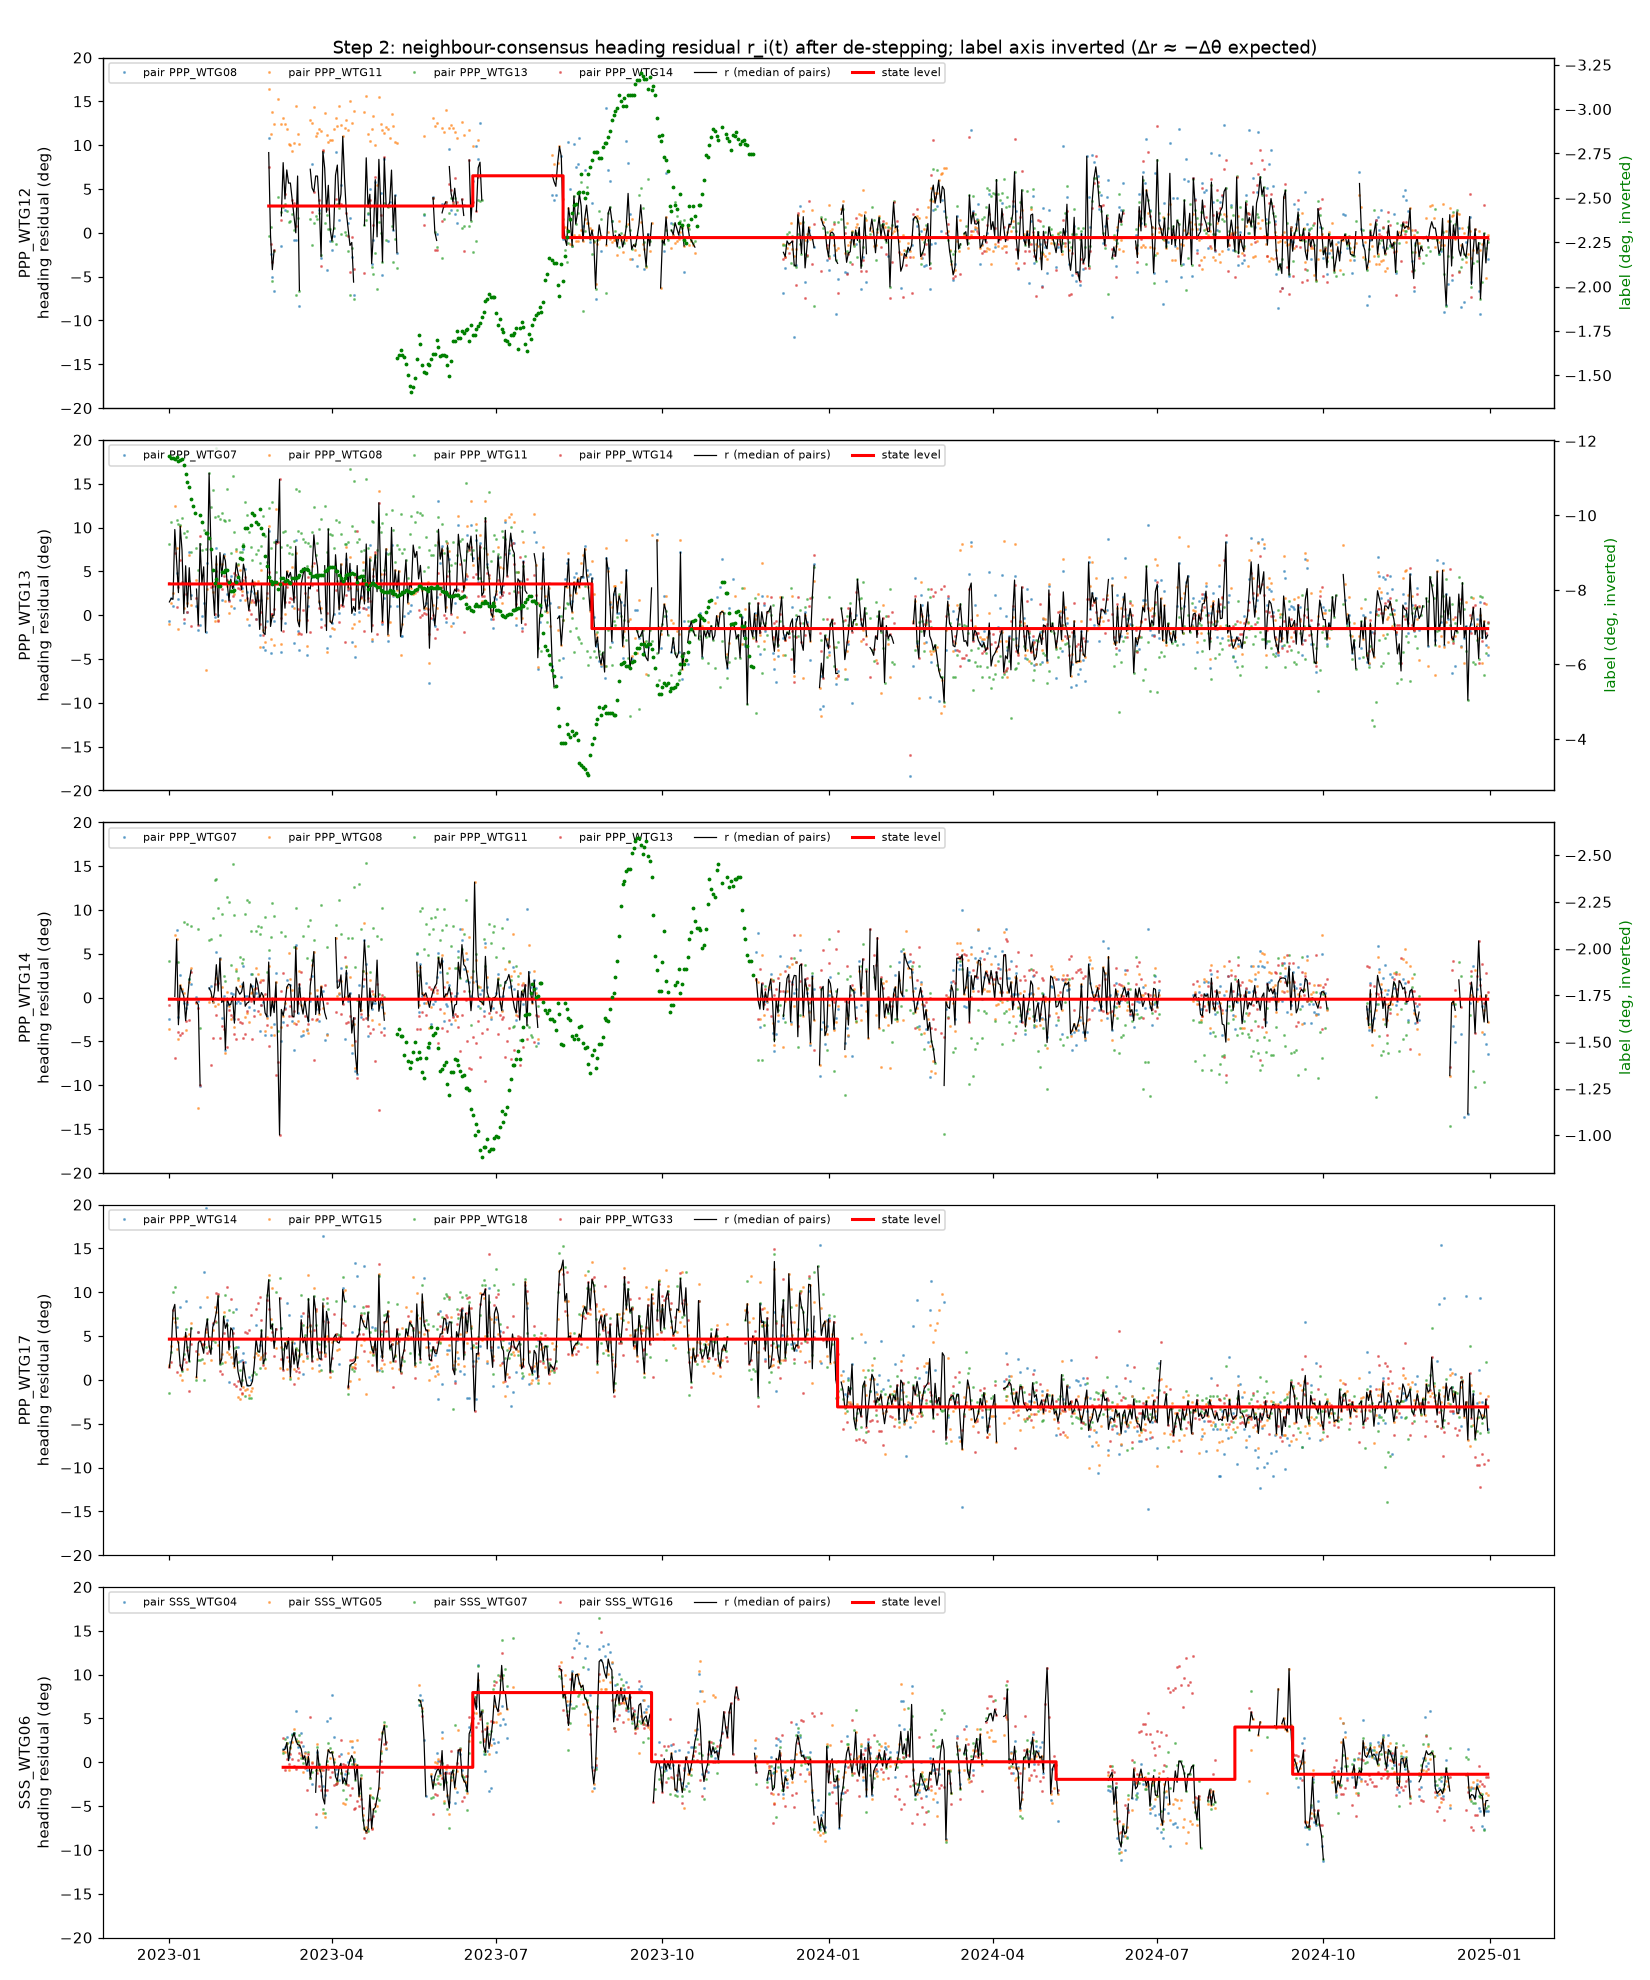
\includegraphics[width=\textwidth]{02_residuals.png}
\caption{Daily pair residuals $e_{ij}(d)$ (coloured dots), their median $r_i(d)$
(black) and the state levels $\bar r_\ell$ (red). On the training turbines the
label is drawn in green on an inverted axis, so that $r$ and the label should
move together by \eqref{eq:dr}.}
\label{fig:residual}
\end{figure}

%======================================================================
\section{The submission model}\label{sec:step4}
\subsection{Structure}
For every turbine-day the prediction is
\begin{equation}
  \hat\theta(d) = L - x(d),\qquad
  x(d) = \bar r_{\ell(d)} - \alpha_{\mathrm{seg}(\ell(d))},
  \label{eq:submission}
\end{equation}
where $\ell(d)$ is the day's SCADA state (\S\ref{sec:states}),
$\mathrm{seg}(\ell)$ its \emph{encoder-free segment} (a maximal run of states
without an encoder-typed boundary, i.e.\ the cumulative count of encoder
boundaries up to $\ell$), $\alpha$ the segment anchor and $L$ the level prior.
The slope of $-1$ on $x$ is \eqref{eq:dr}; no parameter is fitted.
The submitted \code{cluster} field is $\ell(d)$. Days without a SCADA state
(gaps at the record edges) take the nearest state's values; predictions are
rounded to three decimals. The clusters are computed from the residual over
all $731$ days without any knowledge of the template or of which days are
scored; the only calendar prior is $n_{\min}=14$ days.

\subsection{The level prior $L$}
The residual gives changes only; a measured level would have to come from the
turbine's power response to $\gamma$. With the standard empirical law
$P\propto\cos^k\gamma$, $k\approx2$, the power varies by
$\tfrac{k}{2}(8\pi/180)^2\approx2\,\%$ over the $\pm8\dg$ deadband of the yaw
controller, against sector-, turbulence- and season-dependent power variations
of the same order. Estimators of the peak location built on this law were
evaluated in the full project; none survived as a level estimator and none is
used here. The level is therefore a prior, the
\emph{vane set-point}: from \eqref{eq:theta_def} with $g=1$ and the assumption
$\delta_v=0$, $\theta=s$, and $s$ is measured as
\begin{equation}
  L = \med_{d\ \text{healthy}}\ v^{\med}_d ,
  \label{eq:L}
\end{equation}
the median over healthy days of the daily median vane in operation
\eqref{eq:vane_daily}. On the PPP site this is $-2.7$ to $-3.7\dg$ on every
turbine, on SSS $-0.8$ to $-3.3\dg$. The prior is right when the vane is
mounted true and the operator has chosen a non-zero set-point deliberately; it
is wrong by $-\delta_v$ otherwise. On the training turbines it gives biases of
$-1.0$, $+2.3$ and $-1.2\dg$ for the complete model: about a degree on two of
three, and more than two degrees on WTG13, whose vane evidently carries its own
offset.

\subsection{The anchor $\alpha$}
The prior \eqref{eq:L} is a statement about the turbine's \emph{typical} state,
so the state levels must be centred before the slope is applied. Two choices
were evaluated on the training turbines, both taken over the days $d$ of the
segment:
\begin{align}
  \alpha^{\mathrm{med}} &= \med_{d\in\mathrm{seg}} \bar r_{\ell(d)}
  \quad\text{(the level of the state holding most days),}\\
  \alpha^{\mathrm{mean}} &= \frac{1}{|\mathrm{seg}|}\sum_{d\in\mathrm{seg}} \bar r_{\ell(d)}
  \quad\text{(day-weighted average of the state levels).}
\end{align}
The median anchor scores better on train (RMSE $1.91$ versus $2.18$) because the
training turbines have one dominant state. For \code{PPP\_WTG17}, whose two
states hold $370$ and $361$ days, the median anchor is a coin flip that moves the
whole prediction by $4\dg$; the mean anchor minimises the expected squared
error under ignorance of which state is typical, and it was submitted first.
Re-anchoring per segment is what stops re-references below the $25\dg$
attribution threshold of \S\ref{sec:destep} from propagating into the levels.

\subsection{Sign checks}\label{sec:signcheck}
Two independent tests are asserted before any file is written; the script
aborts if either fails.
\begin{enumerate}
\item The least-squares slope of the label on $x$ over the scored training days
      must be negative; measured $-1.07$. This is \eqref{eq:dr} seen from the
      labels.
\item On \code{PPP\_WTG13}, comparing operating samples before 13 January and
      after 19 January 2023, the median vane moved by $-2.6\dg$ while the label
      moved by $+3.0\dg$. By \eqref{eq:theta_def} a change of the set-point (or
      of $\delta_v$ with the controller re-nulling) moves $\theta$ by the same
      amount in the \emph{same} direction, unless the label sign is opposite to
      the raw vane convention. The observed opposite motion therefore fixes the
      label as $-v$ in the raw convention, equivalently as $\gamma=\Wt-\Nt$ once
      the direction in which this controller reports the vane is accounted for.
      The test is asserted as ``vane and label move in opposite directions'' and
      requires $|\Delta v|>1\dg$ and $\Delta\theta^\star>1\dg$.
\end{enumerate}
Together the two tests pin the sign of the submission model, which is all that
matters for scoring.

\subsection{Use of labels}\label{sec:labeluse}
No quantity in \eqref{eq:submission} is fitted to labels: the slope is $-1$ from
\eqref{eq:dr}, the level is \eqref{eq:L} and the states come from the SCADA
residual alone. The training labels enter in two places only: the sign checks
of \S\ref{sec:signcheck}, which fix the sign convention of $\theta$, and the
evaluation of \S\ref{sec:scoring}. The segmentation thresholds
($\lambda$, $n_{\min}$, the $15\dg$ and $25\dg$ limits, the $45$-day excursion
length and the $10\dg$ / $91$-day transient rule) were set while the training
turbines, with their labels, were in view. The frame plan and the transient
rule were introduced after the validate round, when the first final file was
found to disagree with the raw pair offsets of \code{SSS\_WTG06}; the files of
other participants were used to notice the disagreement and to check the
result, not to set a threshold. In particular $\lambda=400$ was kept although
$\lambda=800$ gives three states on \code{SSS\_WTG06}, because it is worse on
the training turbines (RMSE $2.58$ against $2.18$).

\subsection{What was submitted}
\begin{center}\small
\begin{tabular}{@{}llp{3.6cm}p{3.2cm}@{}}
\toprule
file & turbine & states & predicted levels \\
\midrule
\code{Results\_33\_T0\_0.csv} & \code{PPP\_WTG17} & 2 (boundary 2024-01-06, $\Delta r=-7.74\dg$) & $-6.6\dg$ then $+1.1\dg$ \\
\code{Results\_33\_T0\_final.csv} & \code{SSS\_WTG06} & 6, in 1 encoder-free segment & $-8.9\dg\ldots+1.0\dg$, mean $-1.6\dg$ \\
\bottomrule
\end{tabular}
\end{center}
The six levels on \code{SSS\_WTG06} are $-0.4$ (to 2023-06-17), $-8.9$ (to
2023-09-24), $-1.0$ (to 2024-05-05), $+1.0$ (to 2024-08-12), $-5.0$ (to
2024-09-13) and $+0.4\dg$. The \code{PPP\_WTG17} file of the validate round was
produced by the first version of the method ($-6.8$ then $+1.3\dg$); the
present version changes it by at most $0.16\dg$.
Figure~\ref{fig:submission} shows the predictions against the residual they are
derived from.

\begin{figure}[p]\centering
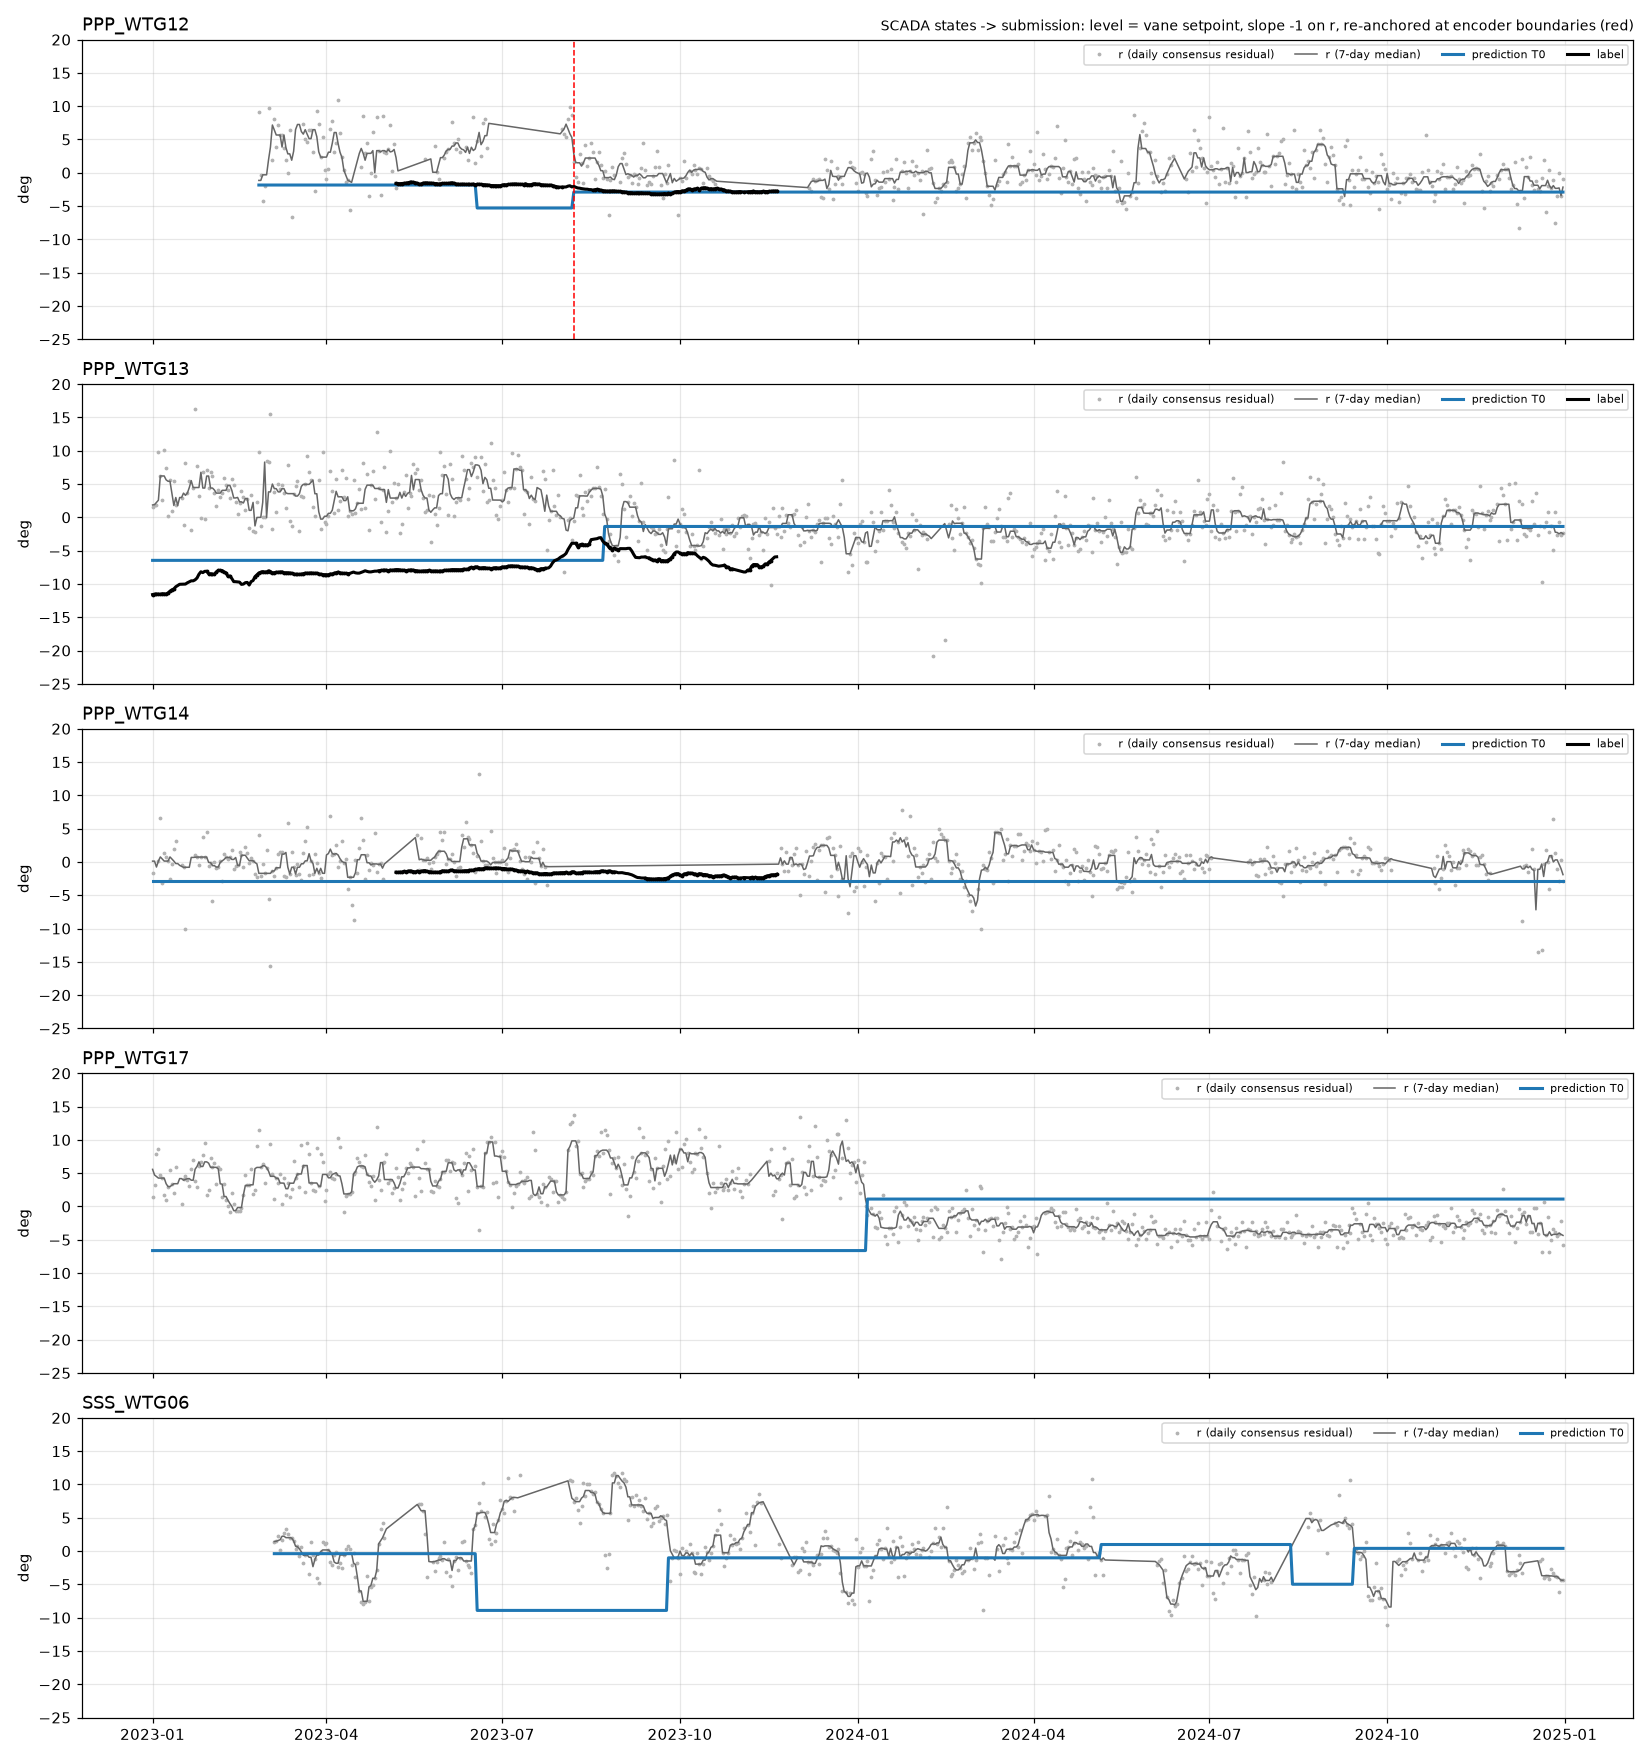
\includegraphics[width=\textwidth]{03_submission.png}
\caption{Daily residual $r$ (grey), T0 prediction $\hat\theta$ (blue) and, on
the training turbines, the label (black). Red dashed lines are encoder-typed
boundaries, across which the prediction is re-anchored.}
\label{fig:submission}
\end{figure}

%======================================================================
\section{Scoring rule and what it rewards}\label{sec:scoring}

\subsection{Metrics}
With $\mathcal D$ the set of scored days (\S\ref{sec:labels}),
\begin{equation}
  \mathrm{RMSE} = \sqrt{\frac1{|\mathcal D|}\sum_{d\in\mathcal D}(\hat\theta_d-\theta^\star_d)^2},\quad
  \mathrm{MAE} = \frac1{|\mathcal D|}\sum_{d\in\mathcal D}|\hat\theta_d-\theta^\star_d|,\quad
  \mathrm{bias} = \frac1{|\mathcal D|}\sum_{d\in\mathcal D}(\hat\theta_d-\theta^\star_d).
\end{equation}
The tie-breaker is the adjusted Rand index between the submitted clusters and
the label-derived states, averaged over turbines. For a contingency table
$n_{uw}$ (cluster $u$, true state $w$) with margins $n_{u\cdot}$, $n_{\cdot w}$
and $n=|\mathcal D|$,
Write $I=\sum_{uw}\binom{n_{uw}}{2}$ for the number of day pairs that
share both a cluster and a true state, $A=\sum_u\binom{n_{u\cdot}}{2}$ and
$B=\sum_w\binom{n_{\cdot w}}{2}$ for the pairs sharing a cluster and sharing a
state respectively, and $E=AB/\binom n2$ for the value of $I$ expected from a
random partition with the same margins. Then
\begin{equation}
  \mathrm{ARI} = \frac{I - E}{\tfrac12(A+B) - E},
\end{equation}
which is $1$ for identical partitions up to relabelling and $0$ in expectation
for a random partition. It is invariant to cluster names; splitting a true state
costs ARI in proportion to the split.

\subsection{Effective sample size and the block bootstrap}
Scored days are runs of a piecewise-constant series, and the error of a
piecewise-constant prediction is constant within each run, so the effective
number of independent observations is the number of states (two on
\code{PPP\_WTG17}, of order fifteen on the training set), not the number of
days. The organisers resample whole states with replacement, score every
submission on the same draw, and call a submission better than another only if
its RMSE is lower on essentially all draws. The local harness reproduces this
with $1000$ draws over (turbine, state) blocks; the resulting $95\,\%$ interval
for the T0 model on the training turbines is $1.5$--$3.1\dg$ around $2.18$,
which is the honest uncertainty of every score quoted in this note.

\subsection{Implication for the strategy}
RMSE differences smaller than that band are ties, and ARI then decides. The
level of $\theta$ cannot be pinned better than a few degrees without labels, so
the winnable quantity is the segmentation (ARI, from \S\ref{sec:step2}) plus a
level that is not badly wrong. The T0 model scores $2.2\dg$ on the training
turbines against a best-constant baseline of $3.1$--$6.1\dg$.

%======================================================================
\section{Summary of assumptions}\label{sec:summary}
\begin{center}\small
\begin{tabular}{@{}lp{3.6cm}p{2.6cm}p{2.4cm}p{4.2cm}@{}}
\toprule
 & measures & units & needs & dominant systematic \\
\midrule
$r$ & $\Delta\theta$ from $\Delta r$ & physical, slope $-1$ & stable $\delta_n$, healthy neighbours & re-references $<15\dg$; neighbour excursions $<10\dg$ \\
$L$ & vane set-point $s$ & physical if $\delta_v=0$ & --- & $\delta_v$ (WTG13: $2.3\dg$) \\
\bottomrule
\end{tabular}
\end{center}

%======================================================================
\section{Outlook: fleet use and further work}\label{sec:outlook}

\subsection{What the method is, operationally}
The method needs the nacelle heading and the power of a turbine and of a few
neighbours from the standard SCADA stream, no labels and no additional sensor,
and processes $16$ turbines over two years in about two minutes. On both
held-out turbines it found the large misalignment changes ($8$--$9\dg$) to
within a day or two, with the step size in physical degrees. That makes it a
candidate for \emph{fleet screening}: a statement of the form ``the alignment
of this turbine changed by about $X\dg$ around this date'', which triggers an
inspection. It is not a replacement for a measurement campaign, for the
reasons below.

\subsection{Weaknesses for a fleet roll-out}
\begin{enumerate}
\item \textbf{No absolute level.} By Proposition~\ref{prop:residual} the
      residual identifies changes only. The level is the prior \eqref{eq:L},
      which is off by $2.3\dg$ on \code{PPP\_WTG13} and cannot be checked
      without a label. A turbine that has been misaligned by a constant amount
      since commissioning is invisible. This is the main gap: closing it with
      one calibration per turbine is exactly the cost the label-free tier is
      meant to avoid.
\item \textbf{Noise floor of several degrees.} The day-to-day noise of $r$ is
      $1$--$2\dg$, but $r$ also wanders by up to $\pm5\dg$ over weeks
      (Figure~\ref{fig:submission}), and with $\lambda=400$ a change needs
      $nJ^2/2\gtrsim400$ to be accepted. Changes below $3$--$5\dg$ are not
      reliable. The training labels only contain changes of $1$--$3\dg$, so
      the range in which the method works is validated on two events
      (\code{PPP\_WTG17}, \code{SSS\_WTG06}) for which no label is available
      to us.
\item \textbf{Dependence on healthy neighbours.} The consensus is a median
      over four pairs. On \code{SSS\_WTG06} two of the four neighbours had
      excursions of their own in August and September 2024, and the file
      contains a $32$-day state at $-5.0\dg$ there that is probably not real.
      Small sites, turbines at the edge of a farm, curtailed or stopped
      neighbours and neighbours that are themselves being re-aligned are weak
      spots; an isolated turbine cannot be assessed at all.
\item \textbf{Encoder events cost data and can hide a change.}
      \code{SSS\_WTG06} loses $117$ of $731$ days to excursions and has a
      residual on $519$ days. A misalignment change that happens during an
      excursion is dated to its end, and one of $15\dg$ or more across an
      excursion is removed as a re-reference. A service visit that changes
      both the vane and the encoder, the most likely real-world cause of a
      misalignment change, is exactly the case in which the two are
      confounded.
\item \textbf{Short states are removed.} The transient rule deletes anything
      shorter than about $45$ days that departs by more than $10\dg$ and
      returns. A real fault of that shape, for example a loose vane that is
      fixed after a month, is not reported.
\item \textbf{Hand-set thresholds.} The $25\dg$, $15\dg$, $10\dg$, $45$-day,
      $91$-day and $\lambda$ values were set on five turbines of one type at
      two sites. The first version failed on the test site for precisely this
      reason: the validate site did not exercise the de-stepping. Other
      controllers, encoder types and terrain have to be expected to break
      some of them.
\item \textbf{Sector correction assumes a stationary site.} The sector
      medians are taken over the whole record. Seasonal stability, vegetation,
      new neighbouring turbines or a changed curtailment strategy move the
      heading difference between two turbines without any misalignment.
\item \textbf{Retrospective.} Centred rolling medians of $7$ and $91$ days and
      a minimum state length of $14$ days mean that a change is confirmed
      about one to two months after it happened. An online version would need
      one-sided windows and would be noisier.
\item \textbf{Changes of the vane gain are invisible.} A change of $\theta$
      through $g$ in \eqref{eq:theta_def} does not move the residual
      (\S\ref{sec:algebra}).
\end{enumerate}

\subsection{Further work}
\begin{enumerate}
\item \textbf{A level estimate.} Combine the residual with a within-turbine,
      encoder-free estimator of the level, for example the power response
      during yaw manoeuvres. Such an estimator is noisy day by day but only
      one number per state is needed: the states of \S\ref{sec:states} say
      which days may be pooled, which is the averaging the power methods lack.
      Alternatively, quantify how many spot calibrations per farm are needed
      when the residual carries the level from one turbine-state to the next.
\item \textbf{Farm-wide solution instead of per-turbine medians.} Every pair
      difference contains the misalignment and the encoder offset of both
      turbines. Solving all pair series of a site jointly, with one
      piecewise-constant offset per turbine and robust weights, would use
      every pair twice, make the attribution of a shift to a turbine explicit
      and remove the fixed choice of four neighbours and the manual reference
      blacklist.
\item \textbf{Segmentation on valid days with a noise model.} PELT currently
      runs on a series interpolated across masked days, so that a gap counts
      as evidence, and with a fixed penalty. Segmenting the valid days only,
      with a penalty scaled by the turbine's own residual noise and its
      autocorrelation, would remove the weak states of 2024 on
      \code{SSS\_WTG06} for a stated reason rather than by tuning $\lambda$.
\item \textbf{Uncertainty per state.} Report an interval for every
      $\Delta\theta$ from the spread across pairs and across days, and a flag
      when a boundary coincides with an excursion of the target or of a
      neighbour. A screening tool needs to say how much to trust each alarm.
\item \textbf{Use the encoder events.} Excursion and re-reference dates are a
      by-product of the frame plan and are themselves maintenance-relevant;
      they also mark the days on which a real change is most likely and least
      observable.
\item \textbf{Validation on more labelled turbines.} The claims above rest on
      three labelled turbines with small steps and two unlabelled ones with
      large steps. Changes of $3$--$10\dg$ with labels, a second turbine
      type and a site with fewer than four neighbours are the missing cases.
\item \textbf{Online operation.} One-sided windows, a detection delay stated
      as a function of the step size, and a false-alarm rate estimated on
      turbines known to be stable.
\end{enumerate}

\end{document}
